\documentclass{standalone}

\usepackage{tikz}
\usetikzlibrary{calc}
\usetikzlibrary{decorations.markings}
\usetikzlibrary{arrows}


\begin{document}
  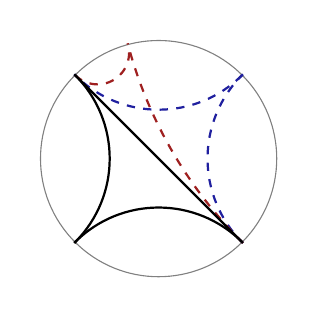
\begin{tikzpicture}

    \begin{scope}[shift={(0,0)},rotate=45]
      \clip (0,0) circle (1.5*1.01) ;
      \draw[gray] (0, 0) circle (1.5*1);

      \draw[dashed, darkgray!50!blue, thick] ( 45:1.5*1.4142) circle (1.5*1);
      \draw[dashed, darkgray!50!blue, thick] (315:1.5*1.4142) circle (1.5*1);

      % Other intercept is at (1/2, sqrt(3)/2)
      \draw[dashed, darkgray!50!red, thick] (1.5*0.267949,1.5* 1) circle (1.5*0.267949);
      \draw[dashed, darkgray!50!red, thick] (1.5*3.73205, 1.5*-1) circle (1.5*3.73205);

      \draw[thick] (135:1.5*(1.4142) circle (1.5*1);
      \draw[thick] (225:1.5*(1.4142) circle (1.5*1);
      \draw[thick] ( 90:1.5*1) -- (270:1.5*1);
    \end{scope}

  \end{tikzpicture}
\end{document}
